\documentclass{beamer}
\usetheme{metropolis}           % Use metropolis theme
\usepackage{arevmath}
\usepackage{varwidth}   
\usepackage{tikz}
\usetikzlibrary{shapes.arrows}
\setsansfont[
	  BoldFont={Fira Sans SemiBold},
	    ItalicFont={Fira Sans BookItalic},
		  BoldItalicFont={Fira Sans SemiBold Italic}
		  ]{Fira Sans Book}
\usepackage{xmpmulti}
\usepackage{graphicx}
\def\shrug{\texttt{\raisebox{0.75em}{\char`\_}\char`\\\char`\_\kern-0.5ex(\kern-0.25ex\raisebox{0.25ex}{\rotatebox{45}{\raisebox{-.75ex}"\kern-1.5ex\rotatebox{-90})}}\kern-0.5ex)\kern-0.5ex\char`\_/\raisebox{0.75em}{\char`\_}}}

\DeclareMathOperator{\dist}{dist}
\newcommand{\light}[1]{\textcolor{gray}{#1}}
\newcommand{\arrowr}{%
\tikz [baseline=-0.5ex]{\node [draw, fill=blue, single arrow, minimum height=3.5ex, rotate=0] {};}}

\title{Efficient Generation of Geographically Accurate Transit Maps}
\date{}
\author{Hannah Bast\,\footnotesize$^1$, \small Patrick Brosi\,\footnotesize$^1$ \small and Sabine Storandt\,\footnotesize$^2$}
\institute{\footnotesize$^1$\,University of Freiburg\\\footnotesize$^2$\,LMU Würzburg\\\\26th ACM SIGSPATIAL - Seattle, Washington, USA}
\begin{document}
\maketitle
\begin{frame}{Motivation}
	\begin{tikzpicture}[overlay]
		\node at (1.5, 3.2) {Official CTA map};
	    \node at (1.5, 0) {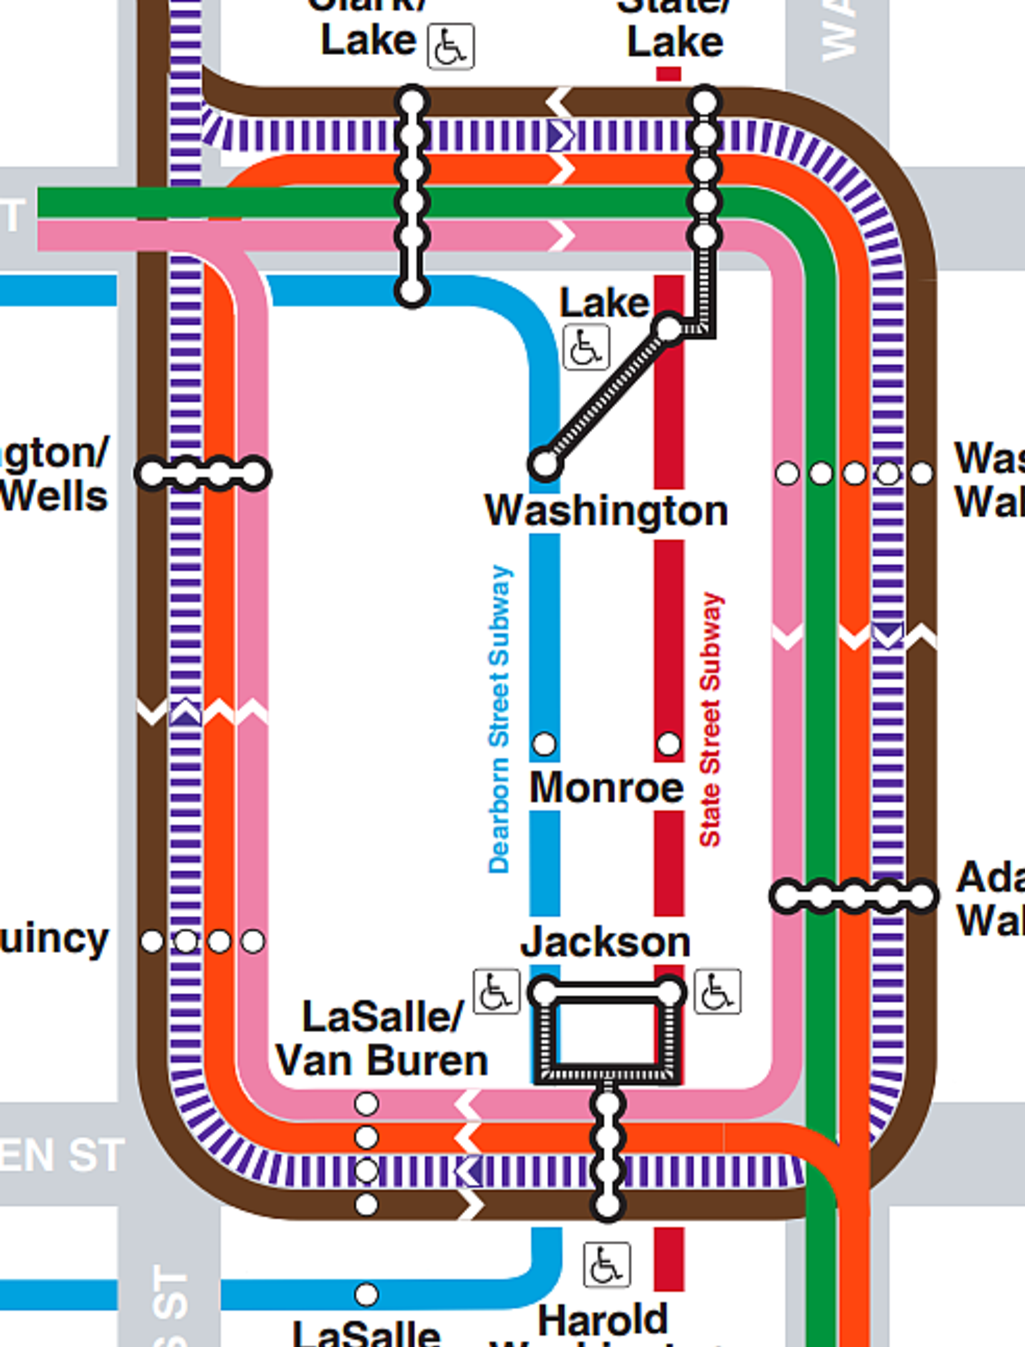
\includegraphics[width=0.3\paperwidth]{figures/chicago_loop.pdf}};
	    \pause
	    \node at (5.5, 3.2) {HERE};
	    \node at (5.5, 0) {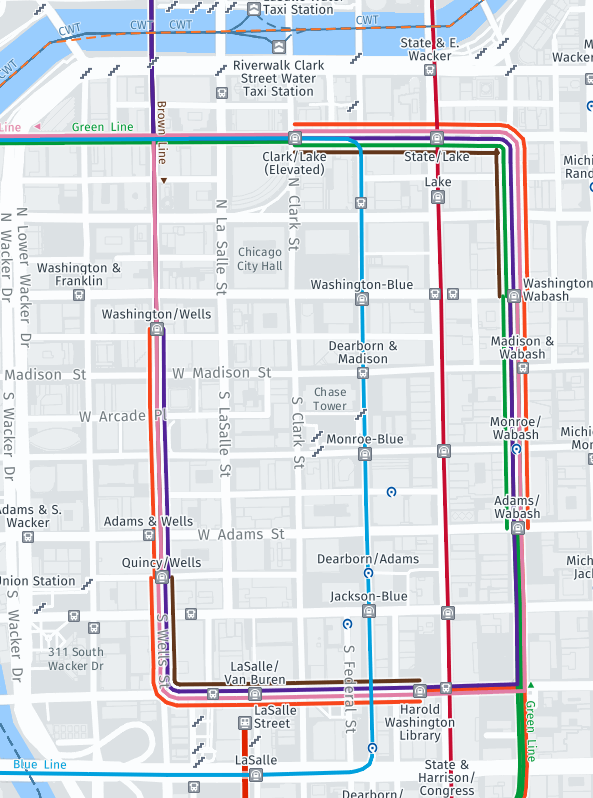
\includegraphics[width=0.3\paperwidth]{figures/chicago_here.png}};
	    \pause
	    \node at (9.5, 3.2) {Google};
	    \node at (9.5, 0) {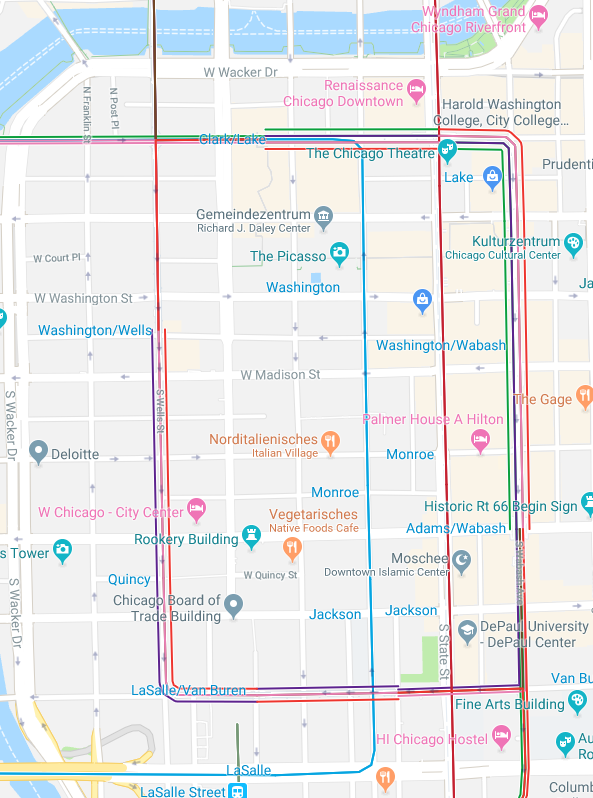
\includegraphics[width=0.3\paperwidth]{figures/chicago_google.png}};
	\end{tikzpicture}
\end{frame}

% --------------------------------------------------------------------------------
\begin{frame}{Goal}
	\textbf{Goal:} Generate these maps \alert{automatically}, in \alert{high quality}

	"Bag of trips"
	\pause
	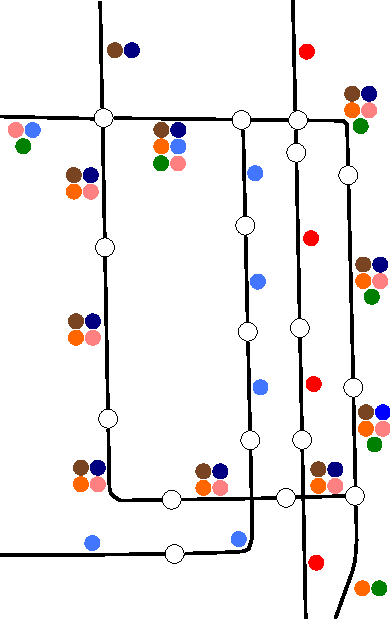
\includegraphics[width=0.25\paperwidth]{figures/chicago_linegraph.pdf}
	\pause
	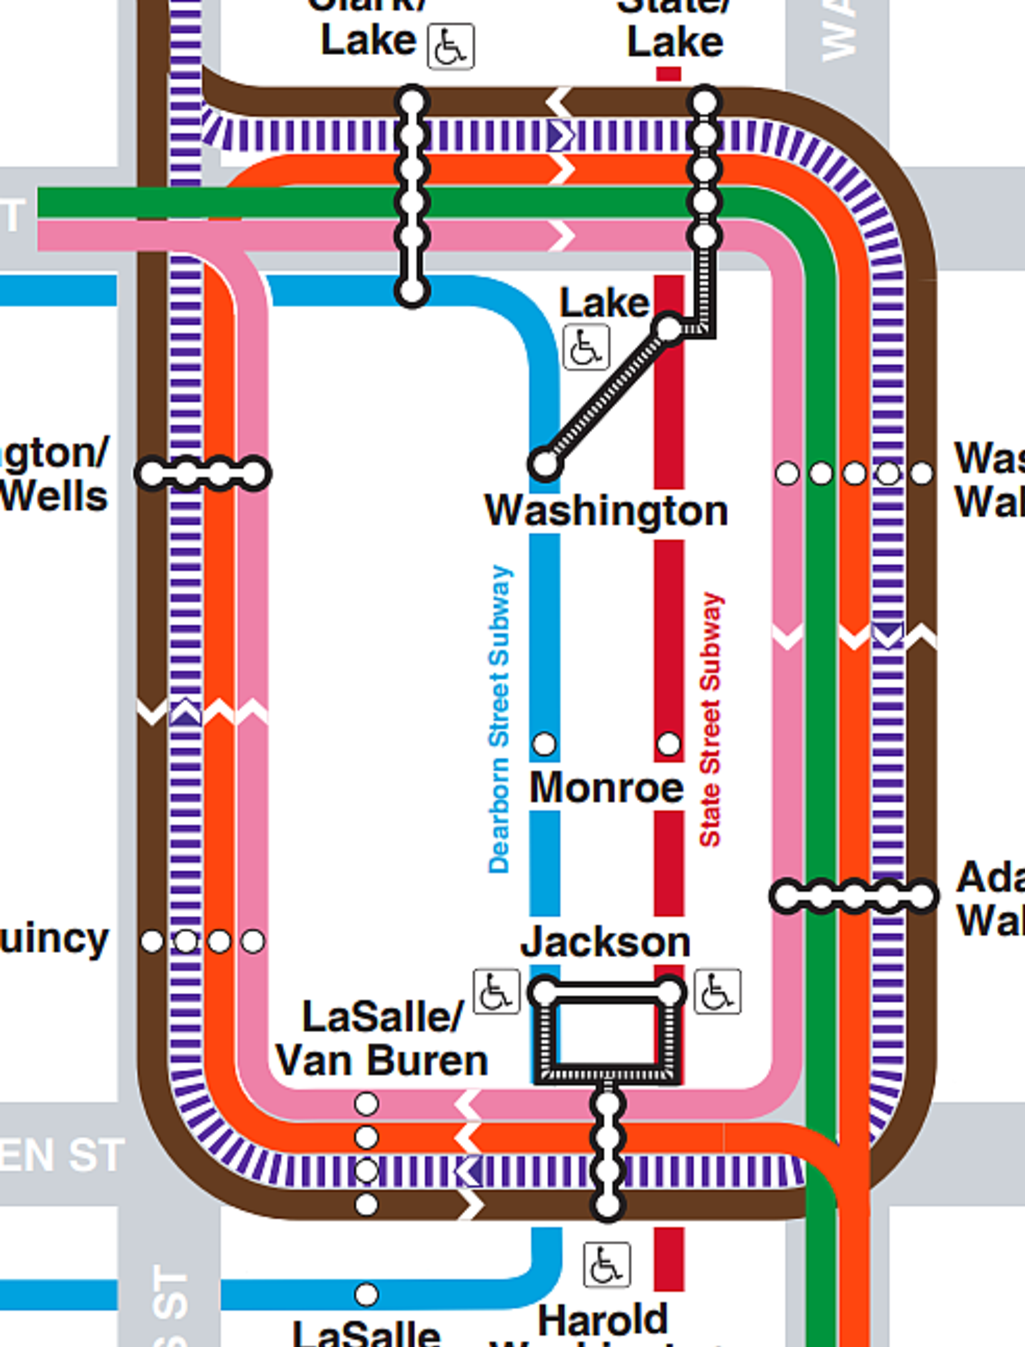
\includegraphics[width=0.25\paperwidth]{figures/chicago_loop.pdf}

\end{frame}

% --------------------------------------------------------------------------------
\begin{frame}{Challenges}
	\begin{tikzpicture}[xshift=.4cm, yshift=.4cm, overlay]
		\begin{scope}[yshift=1.5cm]
			\node at (0.3, 1.6) {\small Official};
			\node at (2.6, 1.6) {\small HERE};
			\node at (4.9, 1.6) {\small Google};

			\node[circle, draw=black!60!green, line width=1.5pt,inner sep=0.7cm, path picture={\node at (path picture bounding box.center) at (-2.09, 1.5) {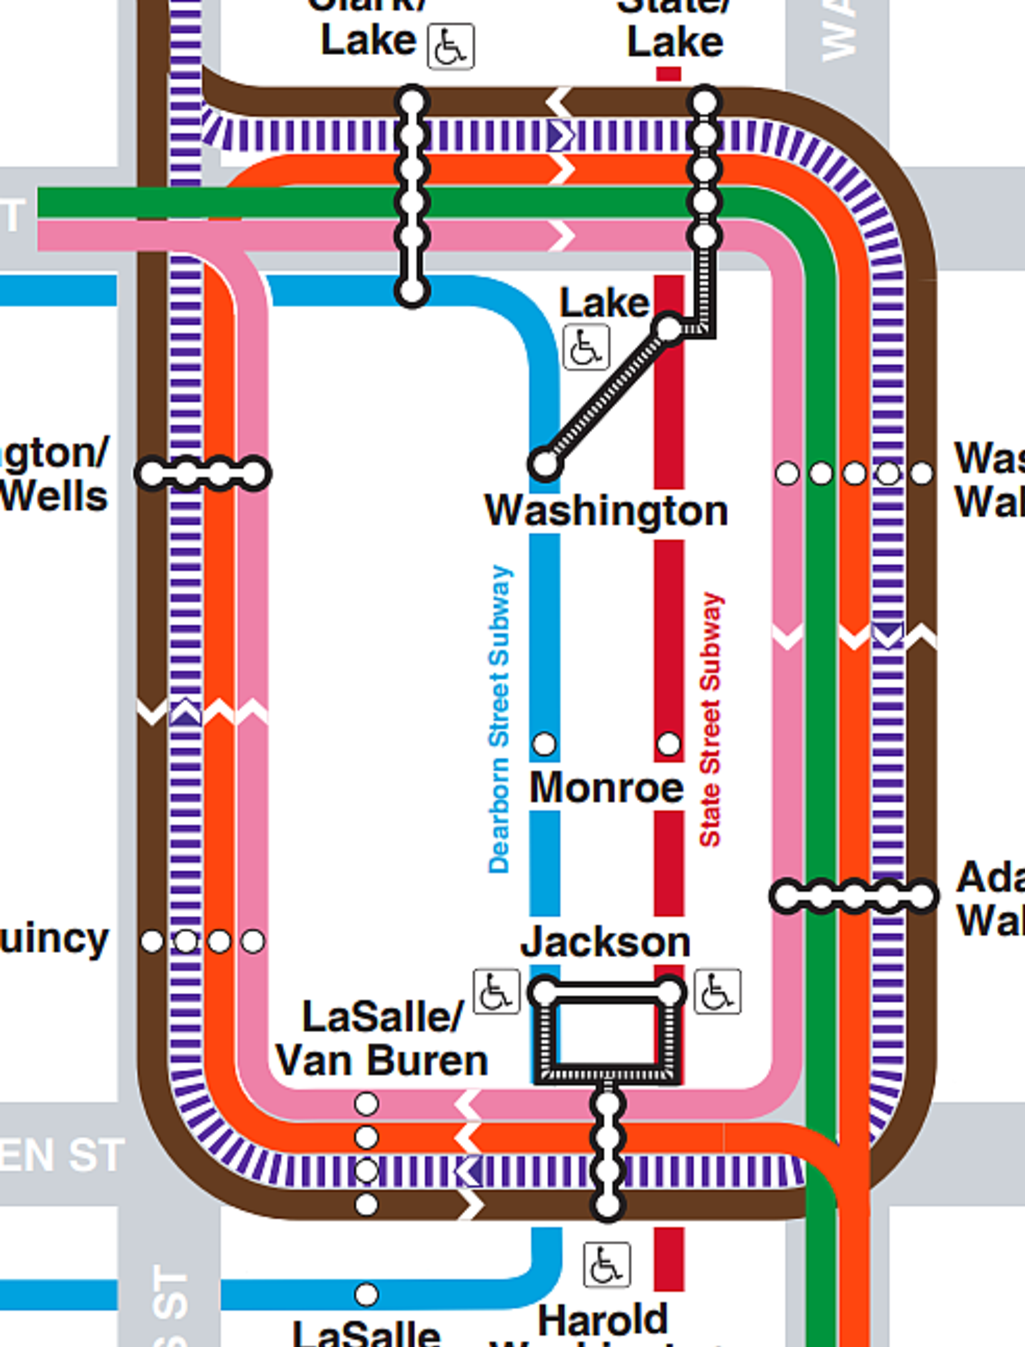
\includegraphics[width=6.5cm]{figures/chicago_loop.pdf}};}] at (0.3, 0) {};
			\node[circle, draw=black!40!red, line width=1.5pt, inner sep=0.7cm, path picture={\node at (path picture bounding box.center) at (-4.45, 3) {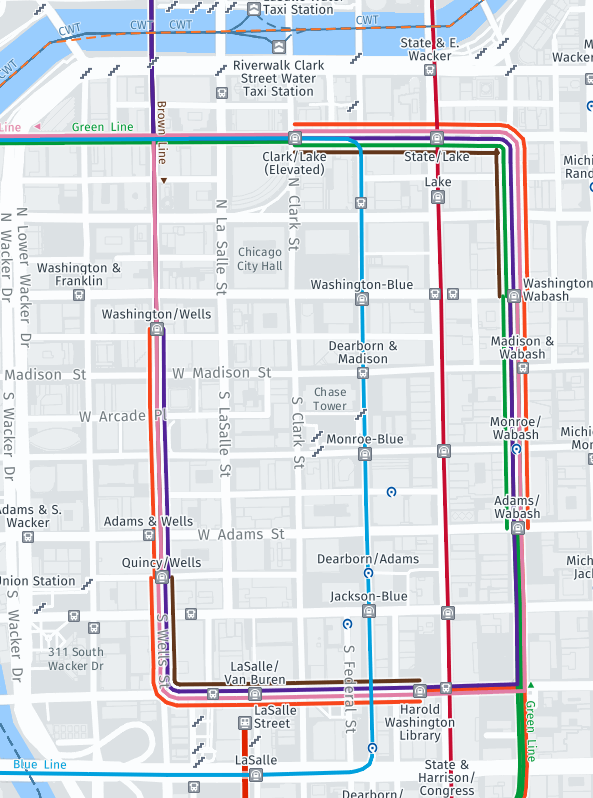
\includegraphics[width=12cm]{figures/chicago_here.png}};}] at (2.6, 0) {};
			\node[circle, draw=black!40!red, line width=1.5pt, inner sep=0.7cm, path picture={\node at (path picture bounding box.center) at (-4.45, 3) {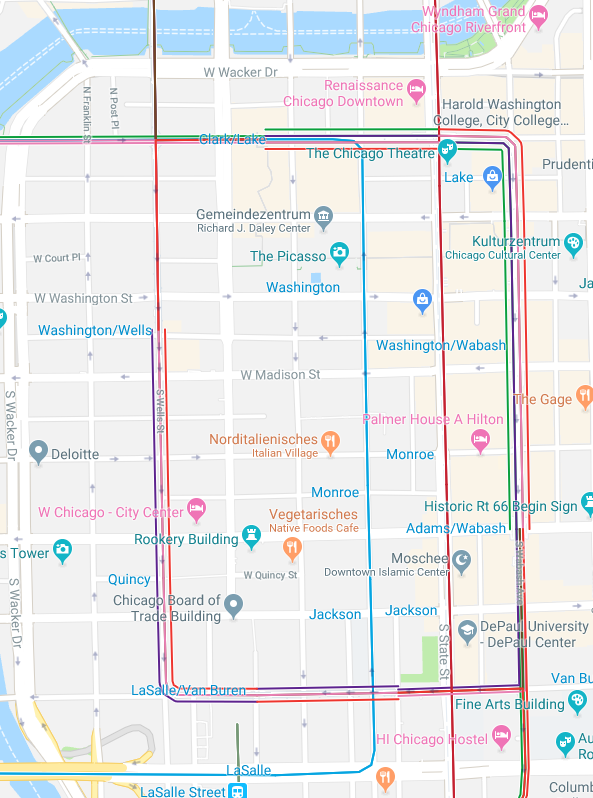
\includegraphics[width=12cm]{figures/chicago_google.png}};}] at (4.9, 0) {};

			\node at (11.5, 0) {
			\vbox{\begin{varwidth}{0.5\textwidth}
				\begin{enumerate}[I.]
					\item Avoid line overlaps
				\end{enumerate}
			\end{varwidth}}};
		\end{scope}

		\pause

		\begin{scope}[yshift=-1.0cm]
			\node[circle, draw=black!60!green, line width=1.5pt, inner sep=0.7cm, path picture={\node at (path picture bounding box.center) at (-1.387, -3.25) {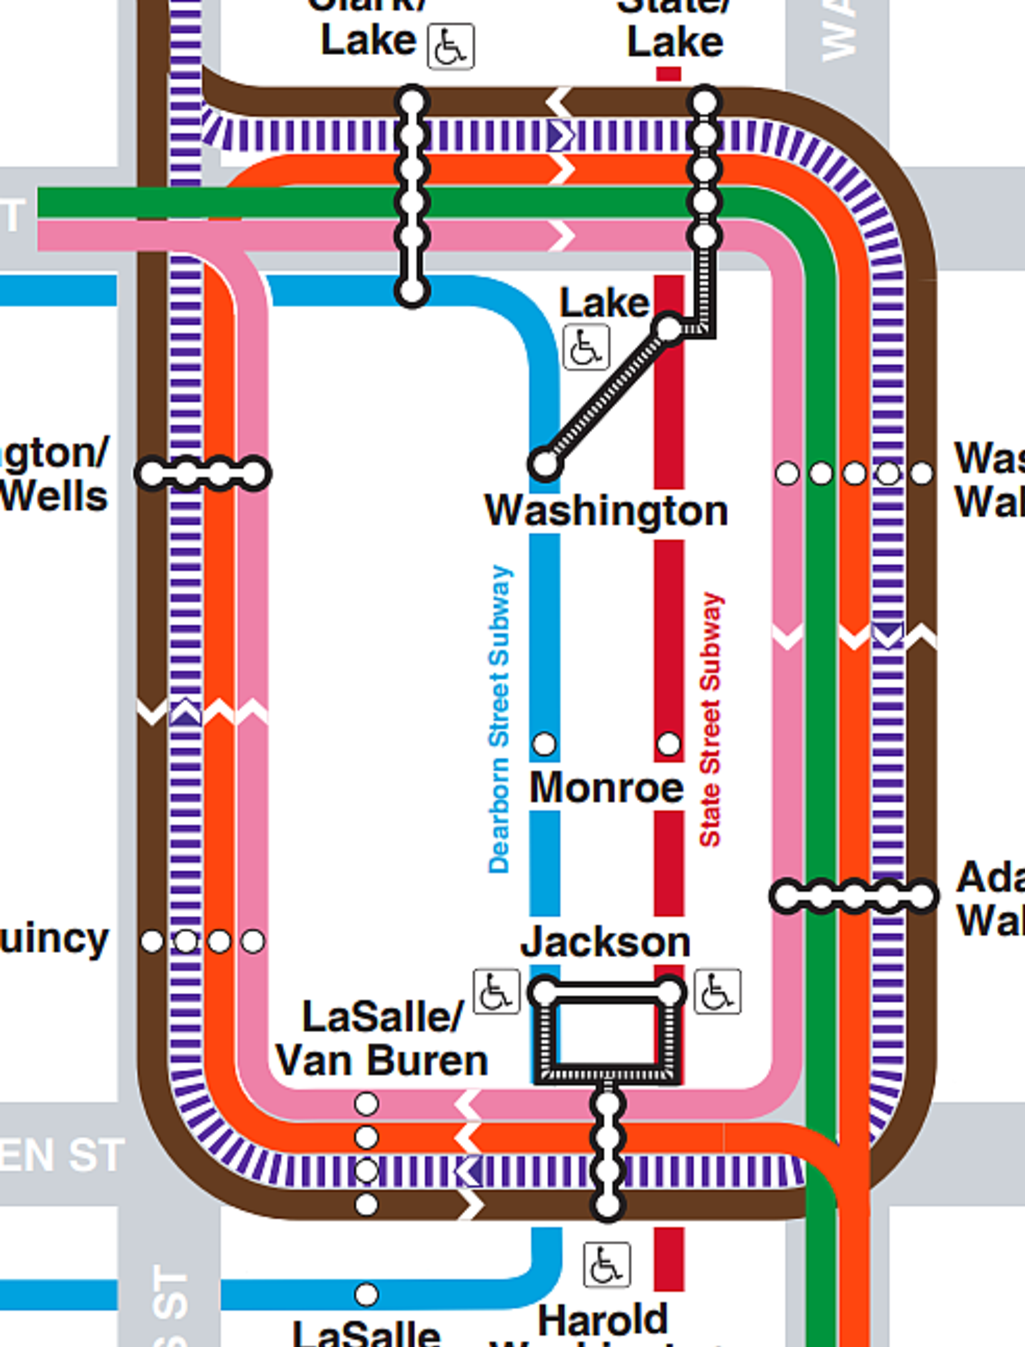
\includegraphics[width=6.75cm]{figures/chicago_loop.pdf}};}] at (0.3, 0) {};
			\node[circle, draw=black!40!red, line width=1.5pt,inner sep=0.7cm, path picture={\node at (path picture bounding box.center) at (-3.75, 8.9) {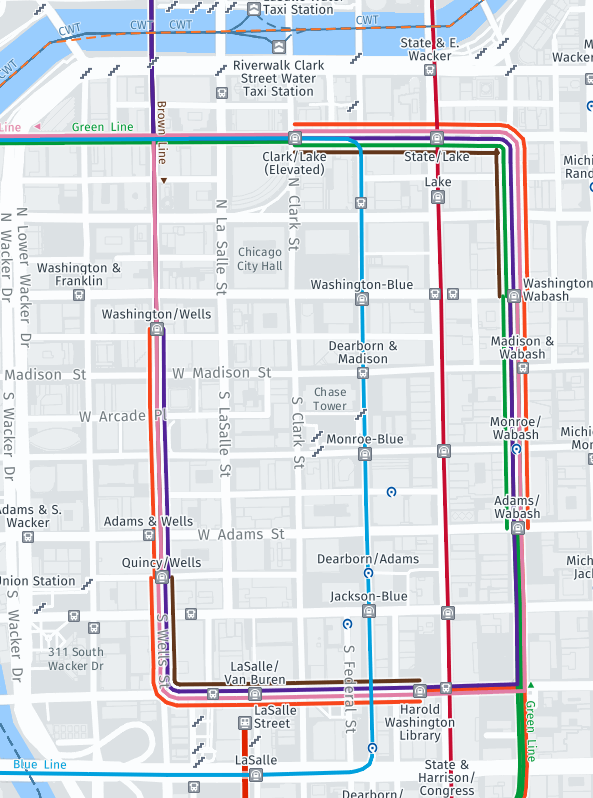
\includegraphics[width=18cm]{figures/chicago_here.png}};}] at (2.6, 0) {};
			\node[circle, draw=black!40!red, line width=1.5pt,inner sep=0.7cm, path picture={\node at (path picture bounding box.center) at (-4.25, -7.9) {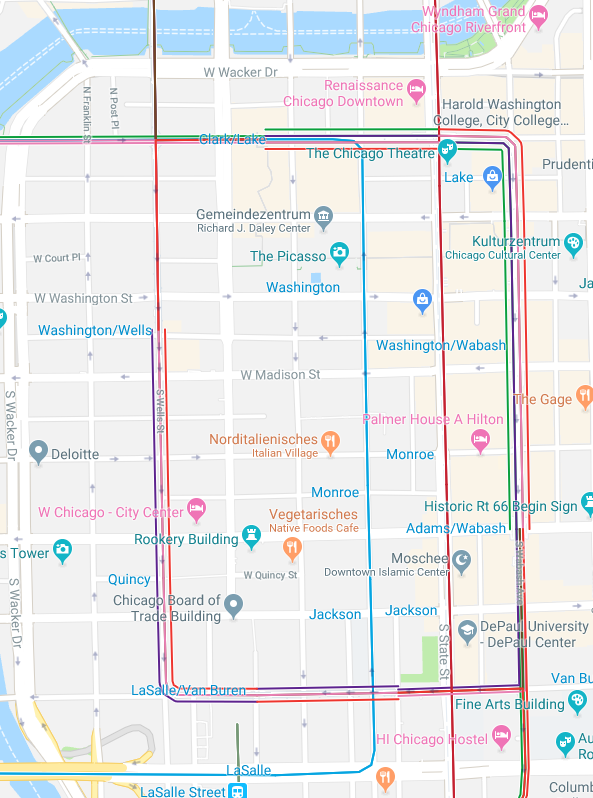
\includegraphics[width=18cm]{figures/chicago_google.png}};}] at (4.9, 0) {};
			\node at (11.5, 0) {
			\vbox{
				\begin{enumerate}[I.]\setcounter{enumi}{1}
					\item Match line orderings
				\end{enumerate}
			}};
		\end{scope}

		\pause

		\begin{scope}[yshift=-3.5cm]
			\node[circle, draw=black!60!green, line width=1.5pt,inner sep=0.7cm, path picture={\node at (path picture bounding box.center) at (-2.03, 2.9) {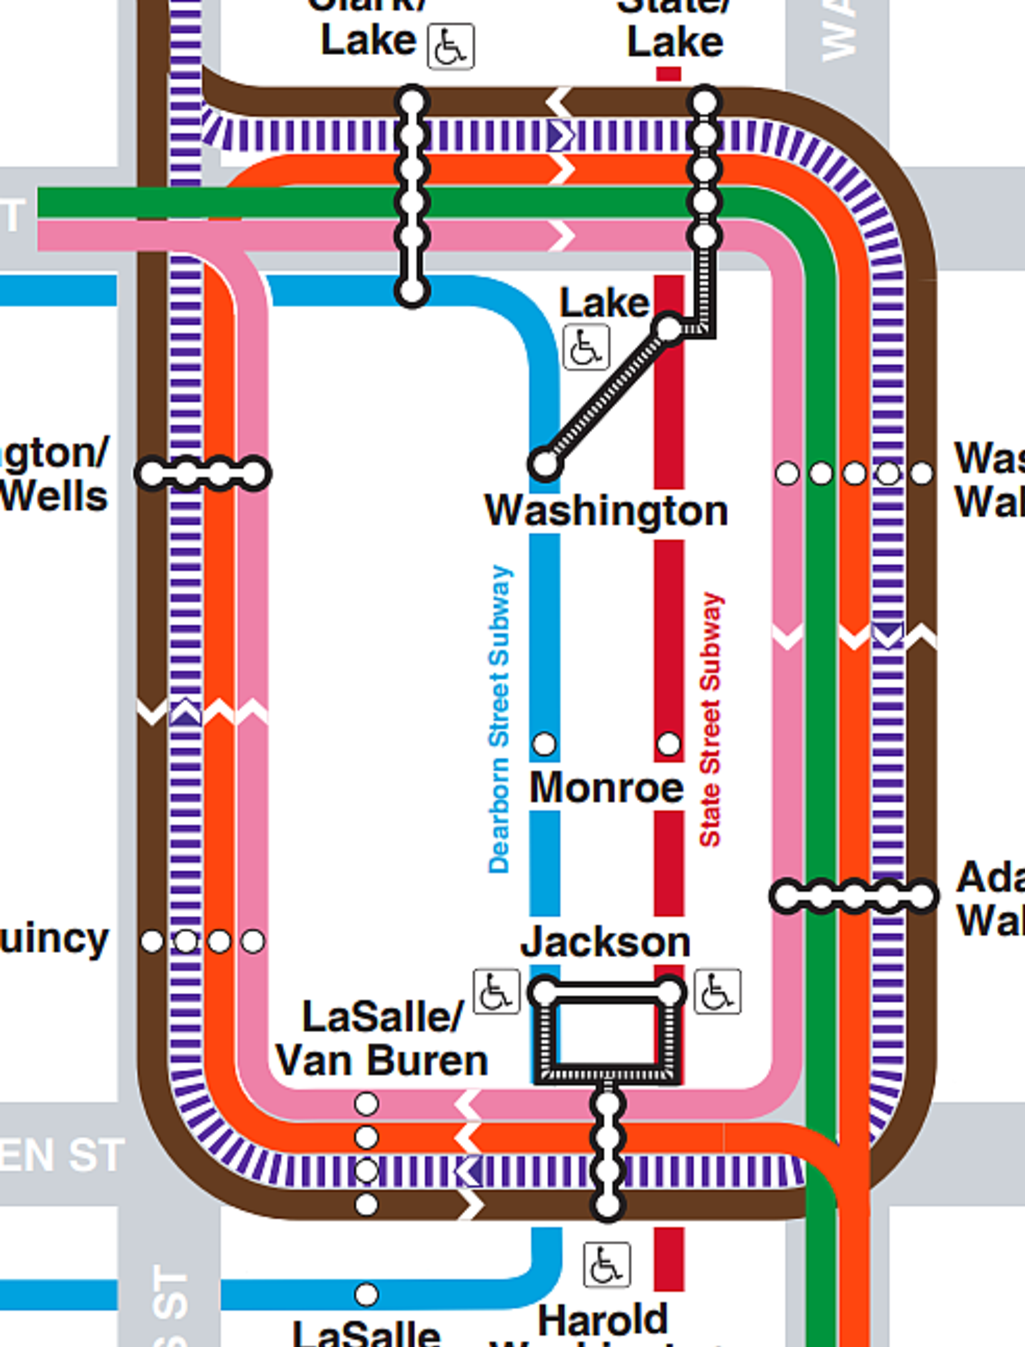
\includegraphics[width=6.5cm]{figures/chicago_loop.pdf}};}] at (0.3, 0) {};
			\node[circle, draw=black!40!red, line width=1.5pt,inner sep=0.7cm, path picture={\node at (path picture bounding box.center) at (-6.75, 8.9) {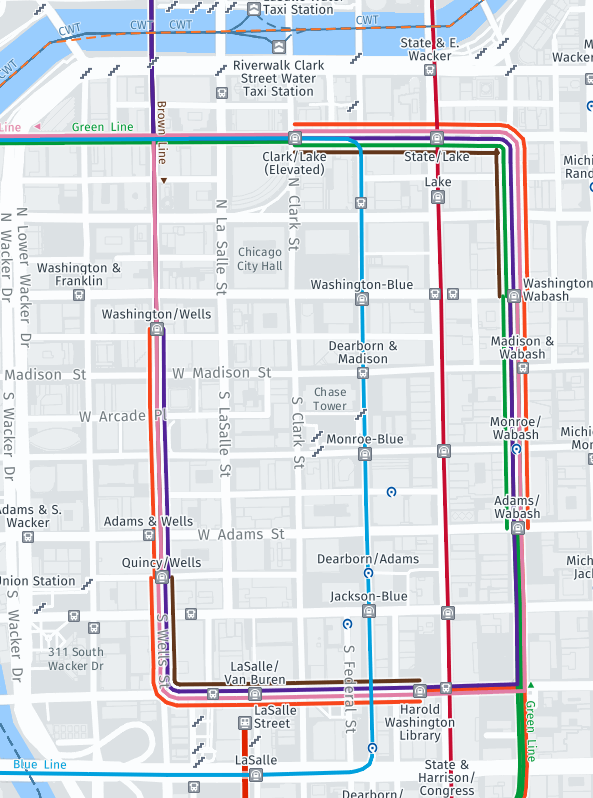
\includegraphics[width=18cm]{figures/chicago_here.png}};}] at (2.6, 0) {};
			\node[circle, draw=black!40!red, line width=1.5pt,inner sep=0.7cm, path picture={\node at (path picture bounding box.center) at (-6.75, 8.9) {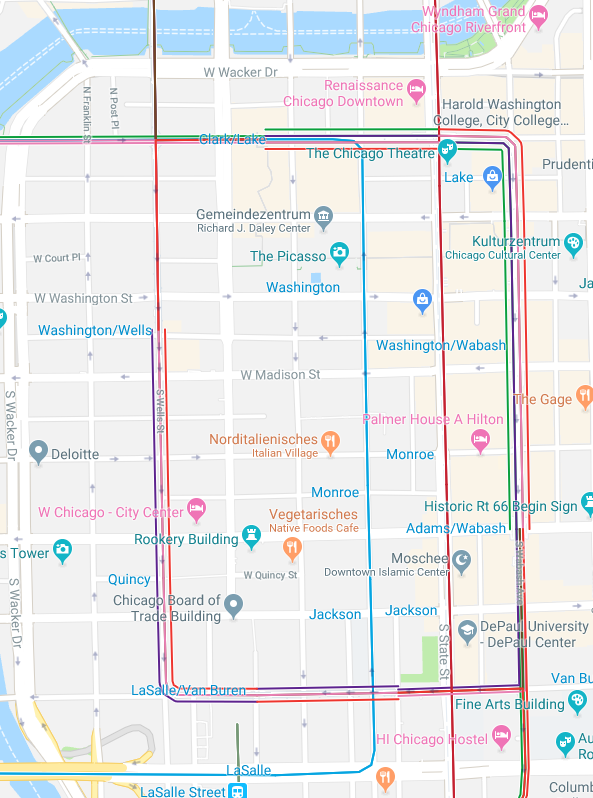
\includegraphics[width=18cm]{figures/chicago_google.png}};}] at (4.9, 0) {};
			\node at (11.5, 0) {
			\vbox{\begin{varwidth}{0.5\textwidth}
				\begin{enumerate}[I.]\setcounter{enumi}{2}
					\item Clearly indicate line continuations
				\end{enumerate}
			\end{varwidth}}};
		\end{scope}
	\end{tikzpicture}
\end{frame}

% --------------------------------------------------------------------------------
\begin{frame}{Line graph construction}
	\begin{columns}[T]
		\begin{column}[T]{0.5\textwidth}
			Line graph:
			\begin{itemize}
				\item Undirected labeled graph $G = (V, E, L)$
				\item Edge labels are subsets of the network lines $\cal L$ ($L(e) \subseteq \cal L$)
				\item Nodes are \alert{usually} stations
			\end{itemize}
		\end{column}
		\begin{column}{0.5\textwidth}
			\centering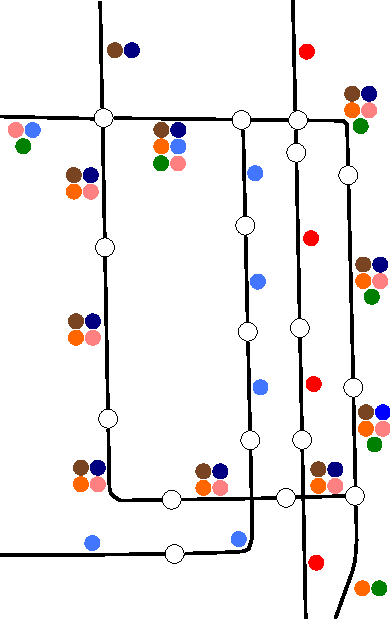
\includegraphics[width=0.6\textwidth]{figures/chicago_linegraph.pdf}
		\end{column}
	\end{columns}


	Example: $\cal L = \{\}$ and $L((a, b)) = \{\}$
\end{frame}

% --------------------------------------------------------------------------------
\begin{frame}{Line graph construction - Input data}
	\only<1> {
		\begin{tikzpicture}[xshift=0cm, yshift=0cm, overlay]
			\node[opacity=1] at (5, -0.2) {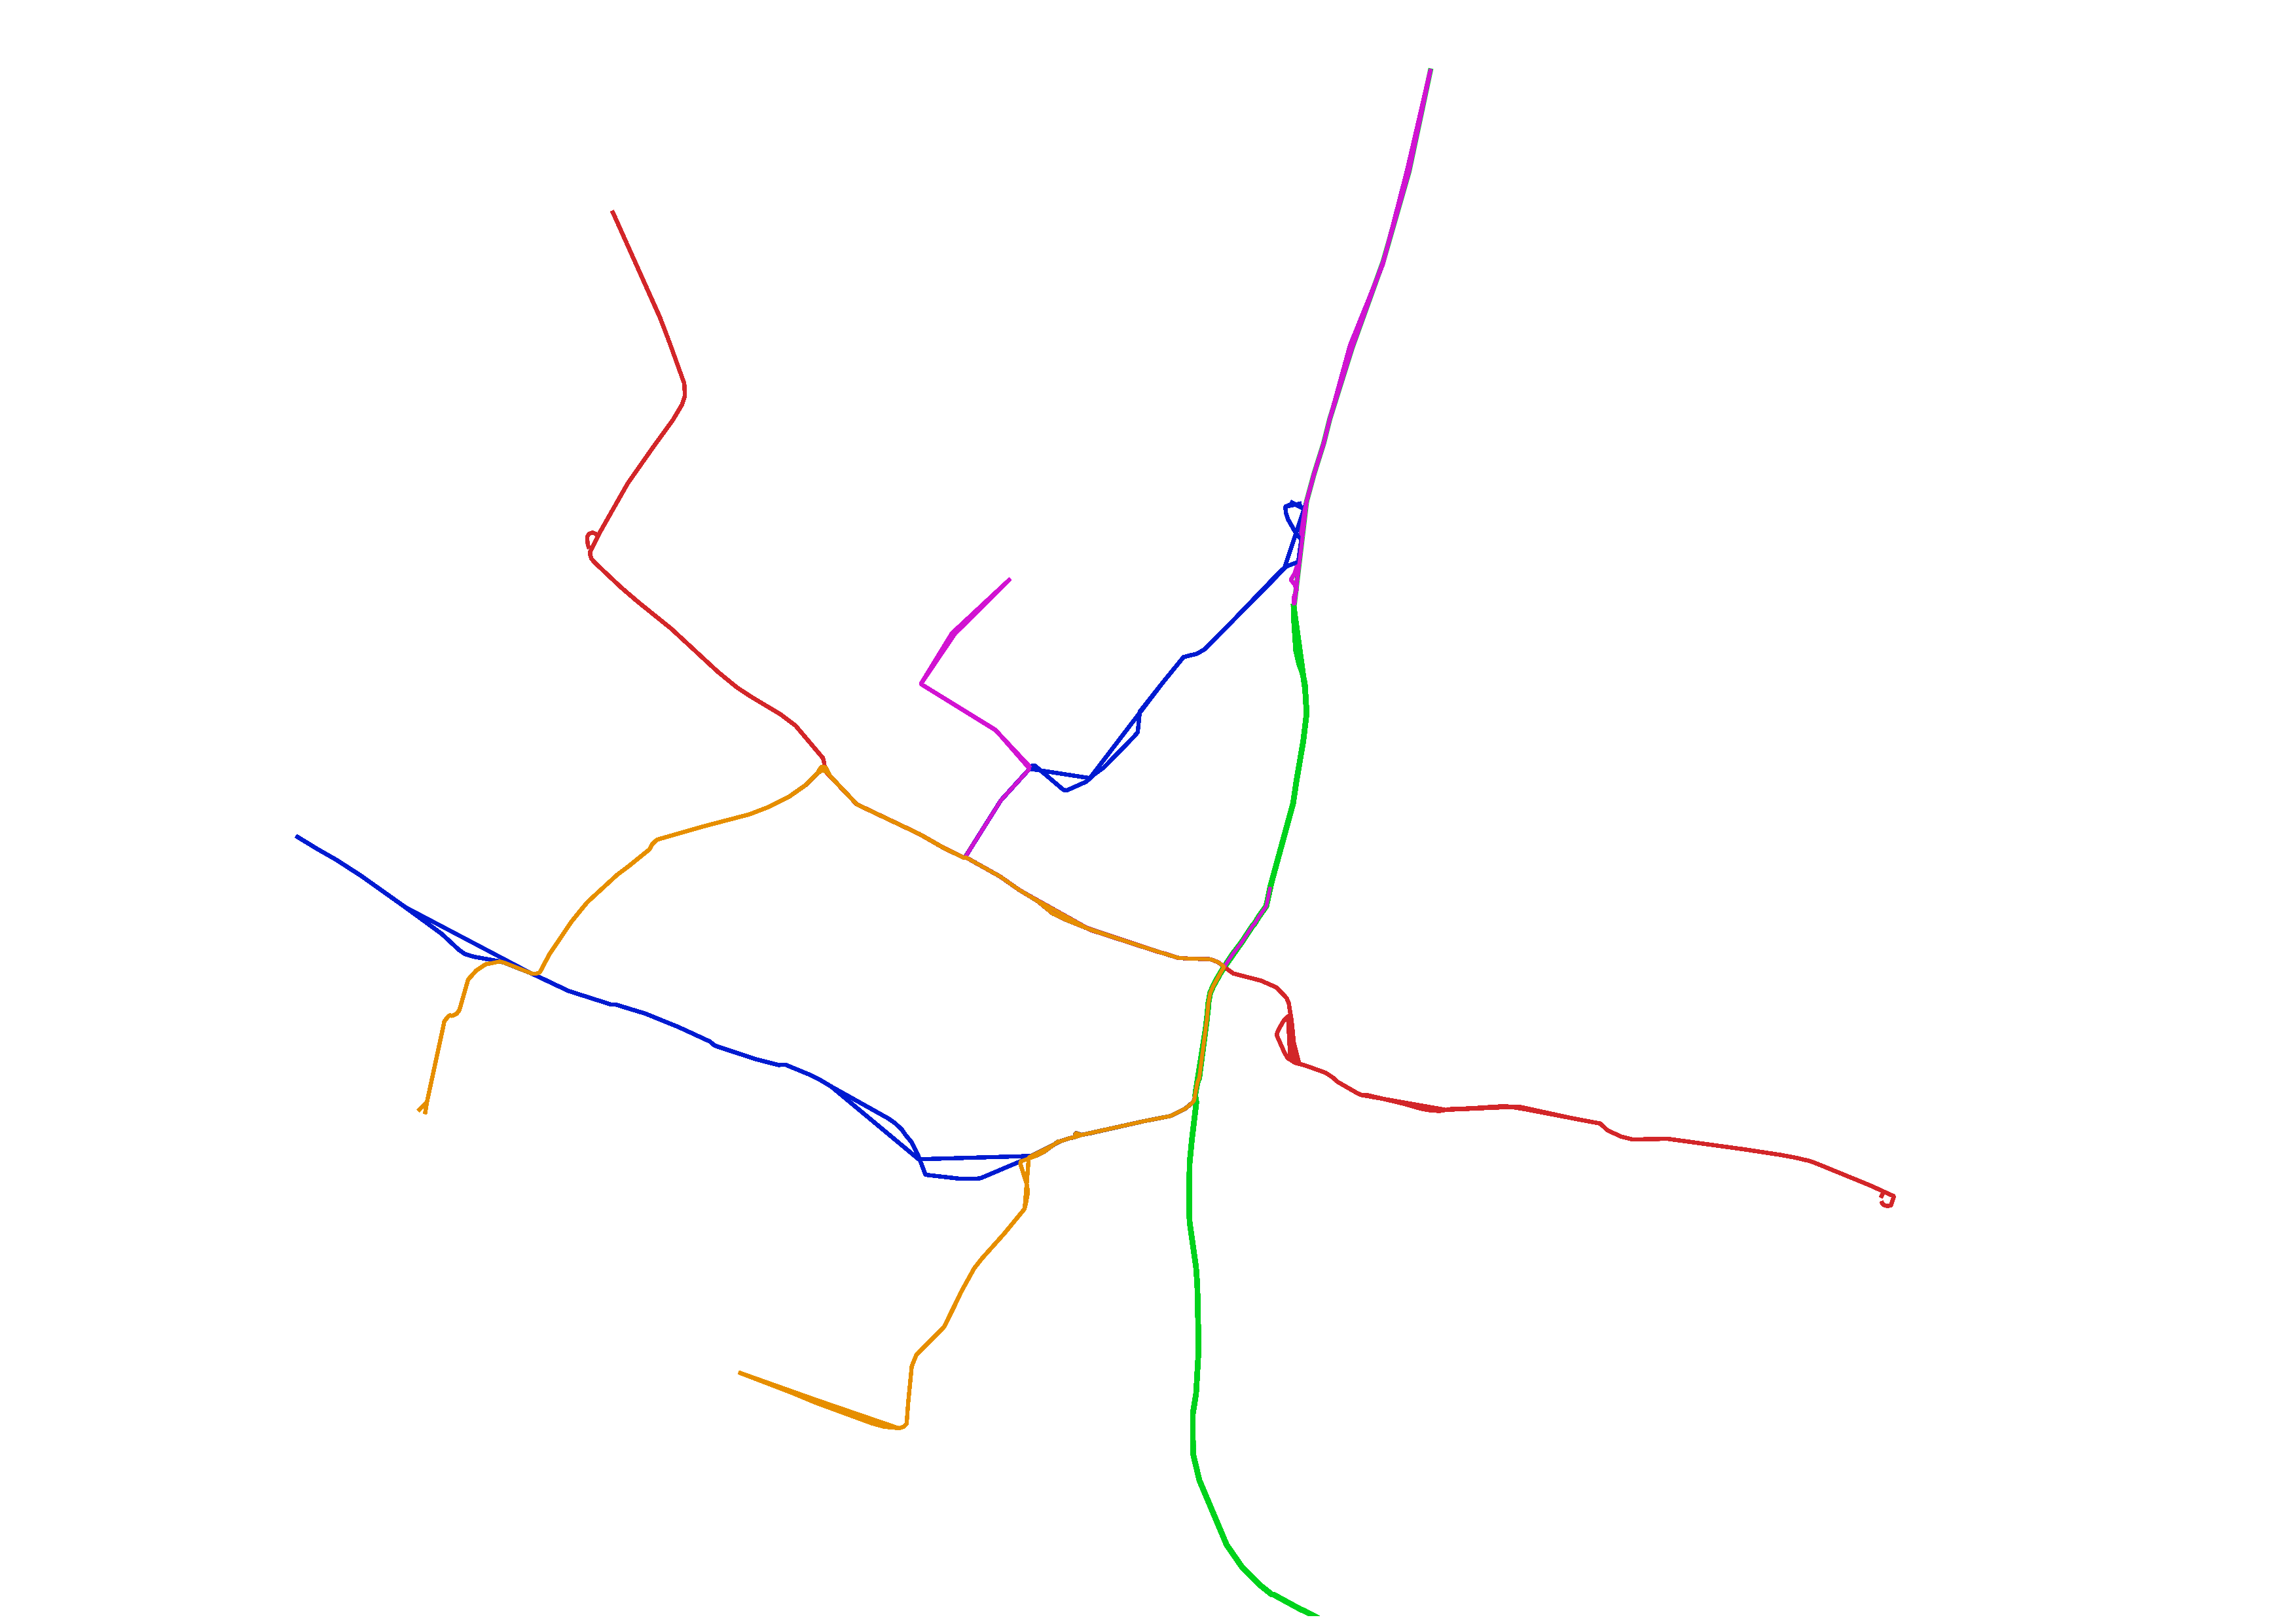
\includegraphics[width=1.1\textwidth]{figures/freiburg_input.png}};
		\end{tikzpicture}
	}
	\only<2>{
		\begin{tikzpicture}[xshift=0cm, yshift=0cm, overlay]


			\draw[line width=0.8pt, draw=gray] (8.9, 2.2) -- (3.3, 0.05);
		\end{tikzpicture}
	}
	\pause
\end{frame}

% --------------------------------------------------------------------------------
\begin{frame}{Line graph construction - Shared segment collapsing}
	\begin{columns}
	    \column{\dimexpr\paperwidth-10pt}

	\centering
	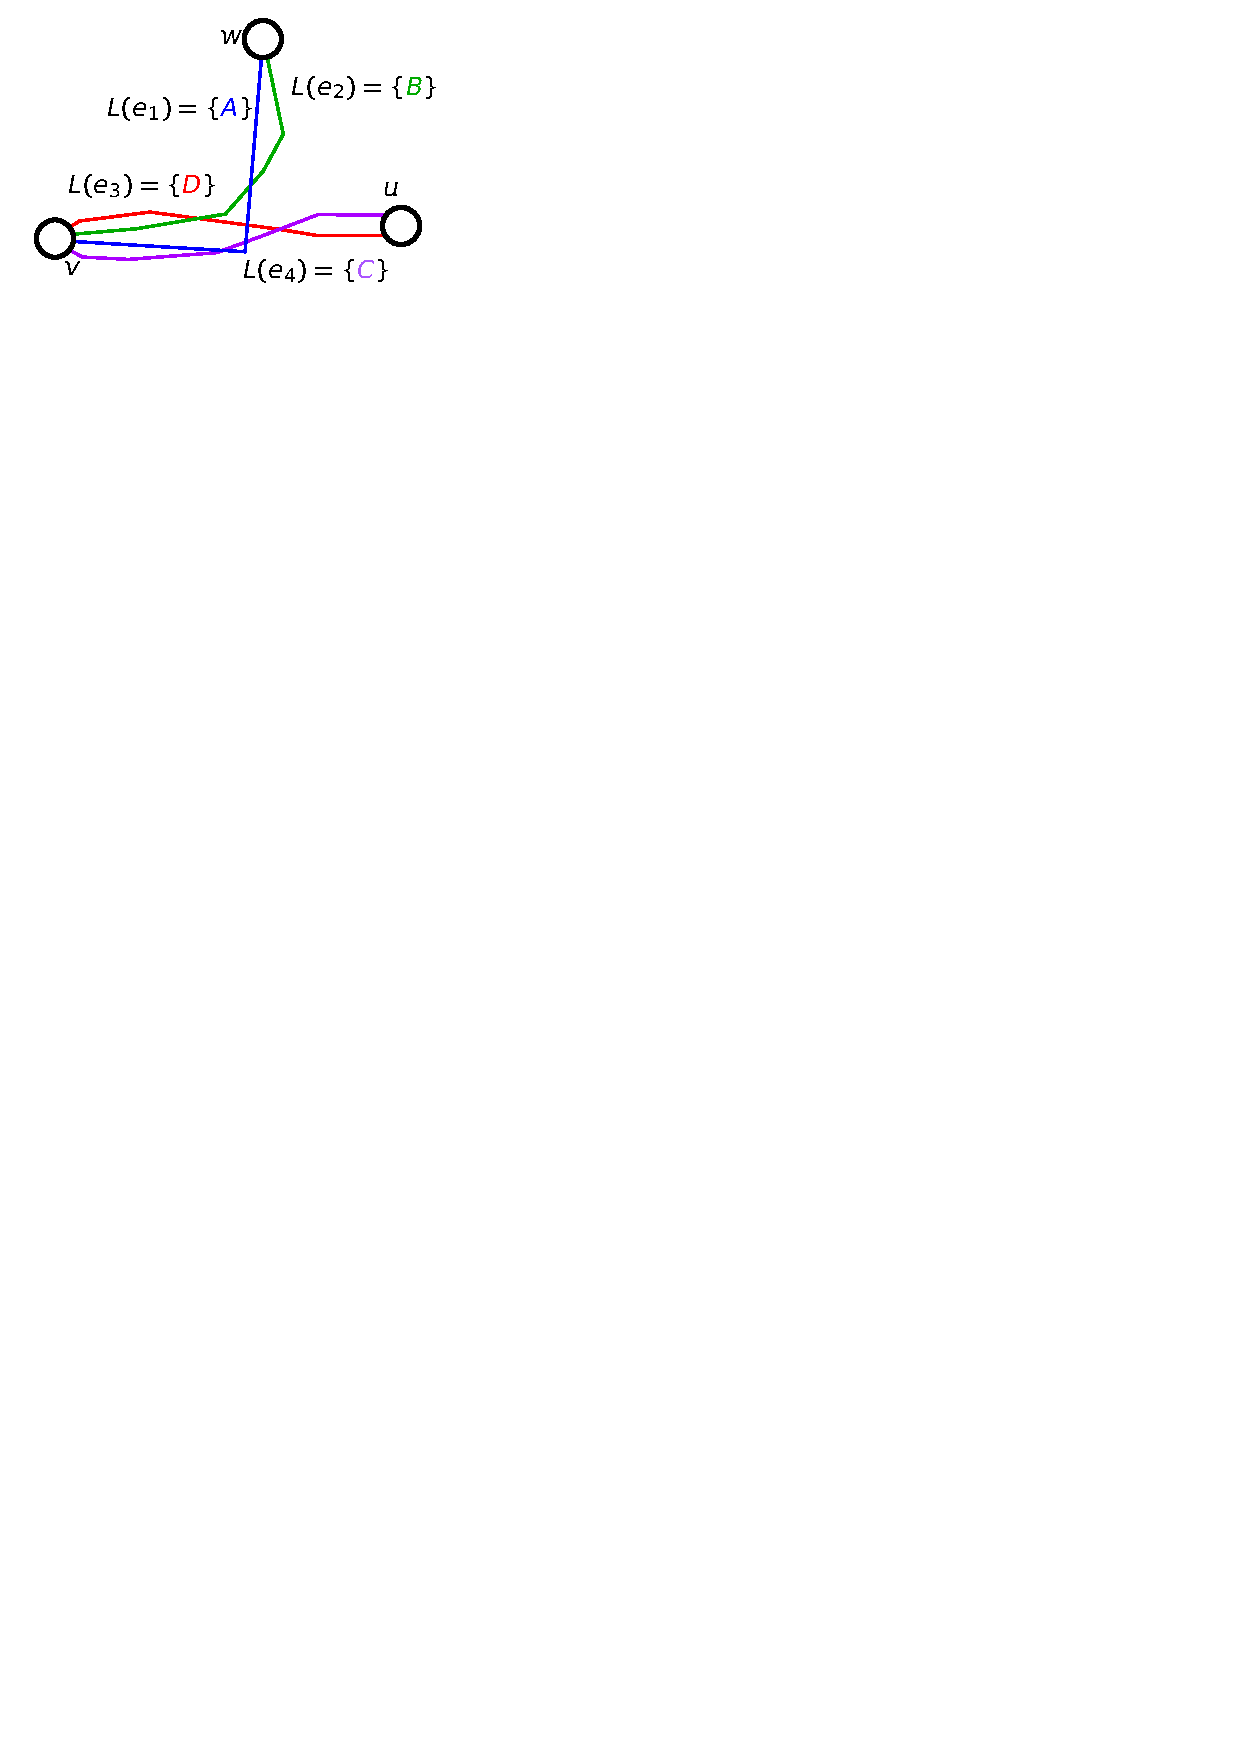
\includegraphics[width=0.3\textwidth,page=1]{figures/linegraph.pdf}
	\includegraphics[width=0.3\textwidth,page=2]{figures/linegraph.pdf}

	\begin{itemize}
		\item Repeatedly collapse (segments of) two edges $e$ and $f$ within a distance $\hat d$
		\item Sweep over some edge $e$ in steps of 10\,m, measure distance $d$ of current point on $e$ to $f$
		\item If $d < \hat d$, start new segment. If not, end current (if open)
		\item Take average between the two "shared segments" on $e$ and $f$
		\item Add \alert{additional non-station nodes} at segment boundaries
	\end{itemize}

	\end{columns}
\end{frame}

% --------------------------------------------------------------------------------
\begin{frame}{Line graph construction - Why non-station nodes?}
	$\begin{array}{l}\includegraphics[width=0.4\textwidth,page=3]{figures/linegraph.pdf}\end{array}$
	\pause
	\arrowr
	$\begin{array}{l}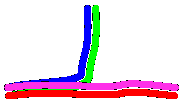
\includegraphics[width=0.4\textwidth]{figures/example.pdf}\end{array}$
	\pause
	\vfill

	$\begin{array}{l}\includegraphics[width=0.4\textwidth,page=2]{figures/linegraph.pdf}\end{array}$
	\pause
	\arrowr
	$\begin{array}{l}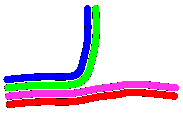
\includegraphics[width=0.4\textwidth]{figures/example2.pdf}\end{array}$
\end{frame}

% --------------------------------------------------------------------------------
\begin{frame}{Results so far (1)}
	\only<1>{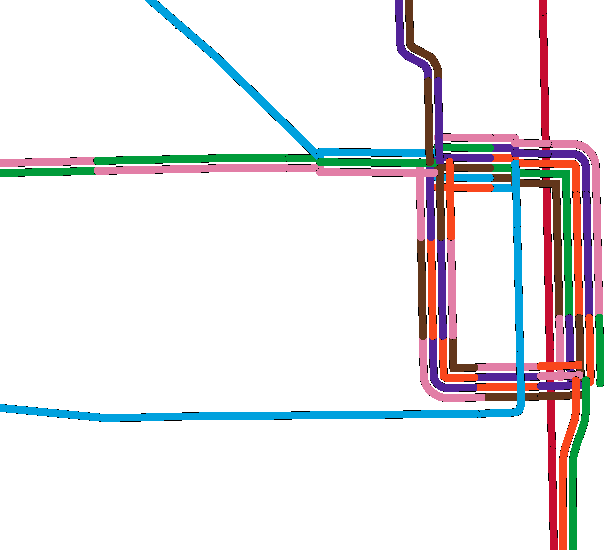
\includegraphics[width=0.8\textwidth]{figures/interim1.pdf}}
	\pause
	\only<2>{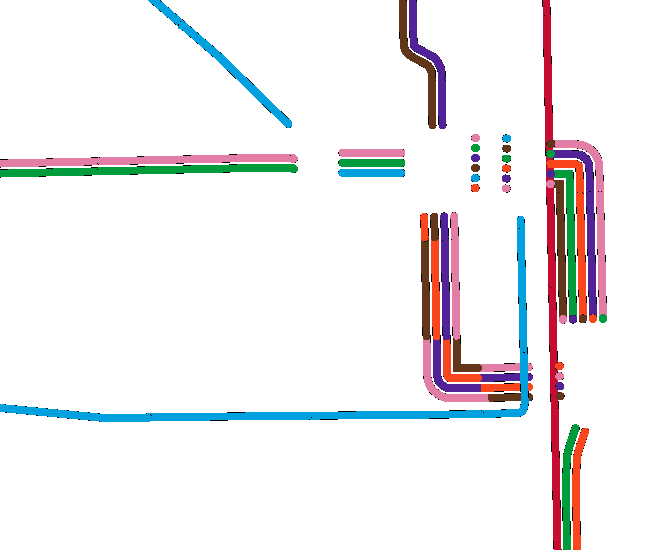
\includegraphics[width=0.861\textwidth]{figures/interim2.pdf}}
\end{frame}

% --------------------------------------------------------------------------------
\begin{frame}{Line-ordering optimization}
	\begin{columns}[T]
		\begin{column}{0.3\textwidth}
			\centering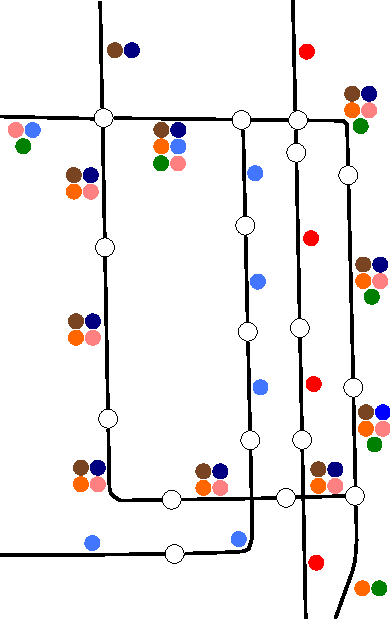
\includegraphics[width=1\textwidth]{figures/chicago_linegraph.pdf}
		\end{column}
		\begin{column}[T]{0.7\textwidth}			
			\begin{itemize}
				\item 23 edges
				\item Each edge $e$ has $|L(e)|!$ possible line permutations
				\item Possible configurations for the graph on the left: \alert{$> 2\times 10^{17}$}
			\end{itemize}
			\textbf{$\Rightarrow$ Naive exhaustive search infeasible}
		\end{column}
	\end{columns}
\end{frame}

% --------------------------------------------------------------------------------
\begin{frame}{Line-ordering optimization - Baseline ILP}
	\begin{columns}[T]
		\begin{column}{0.25\textwidth}
			\centering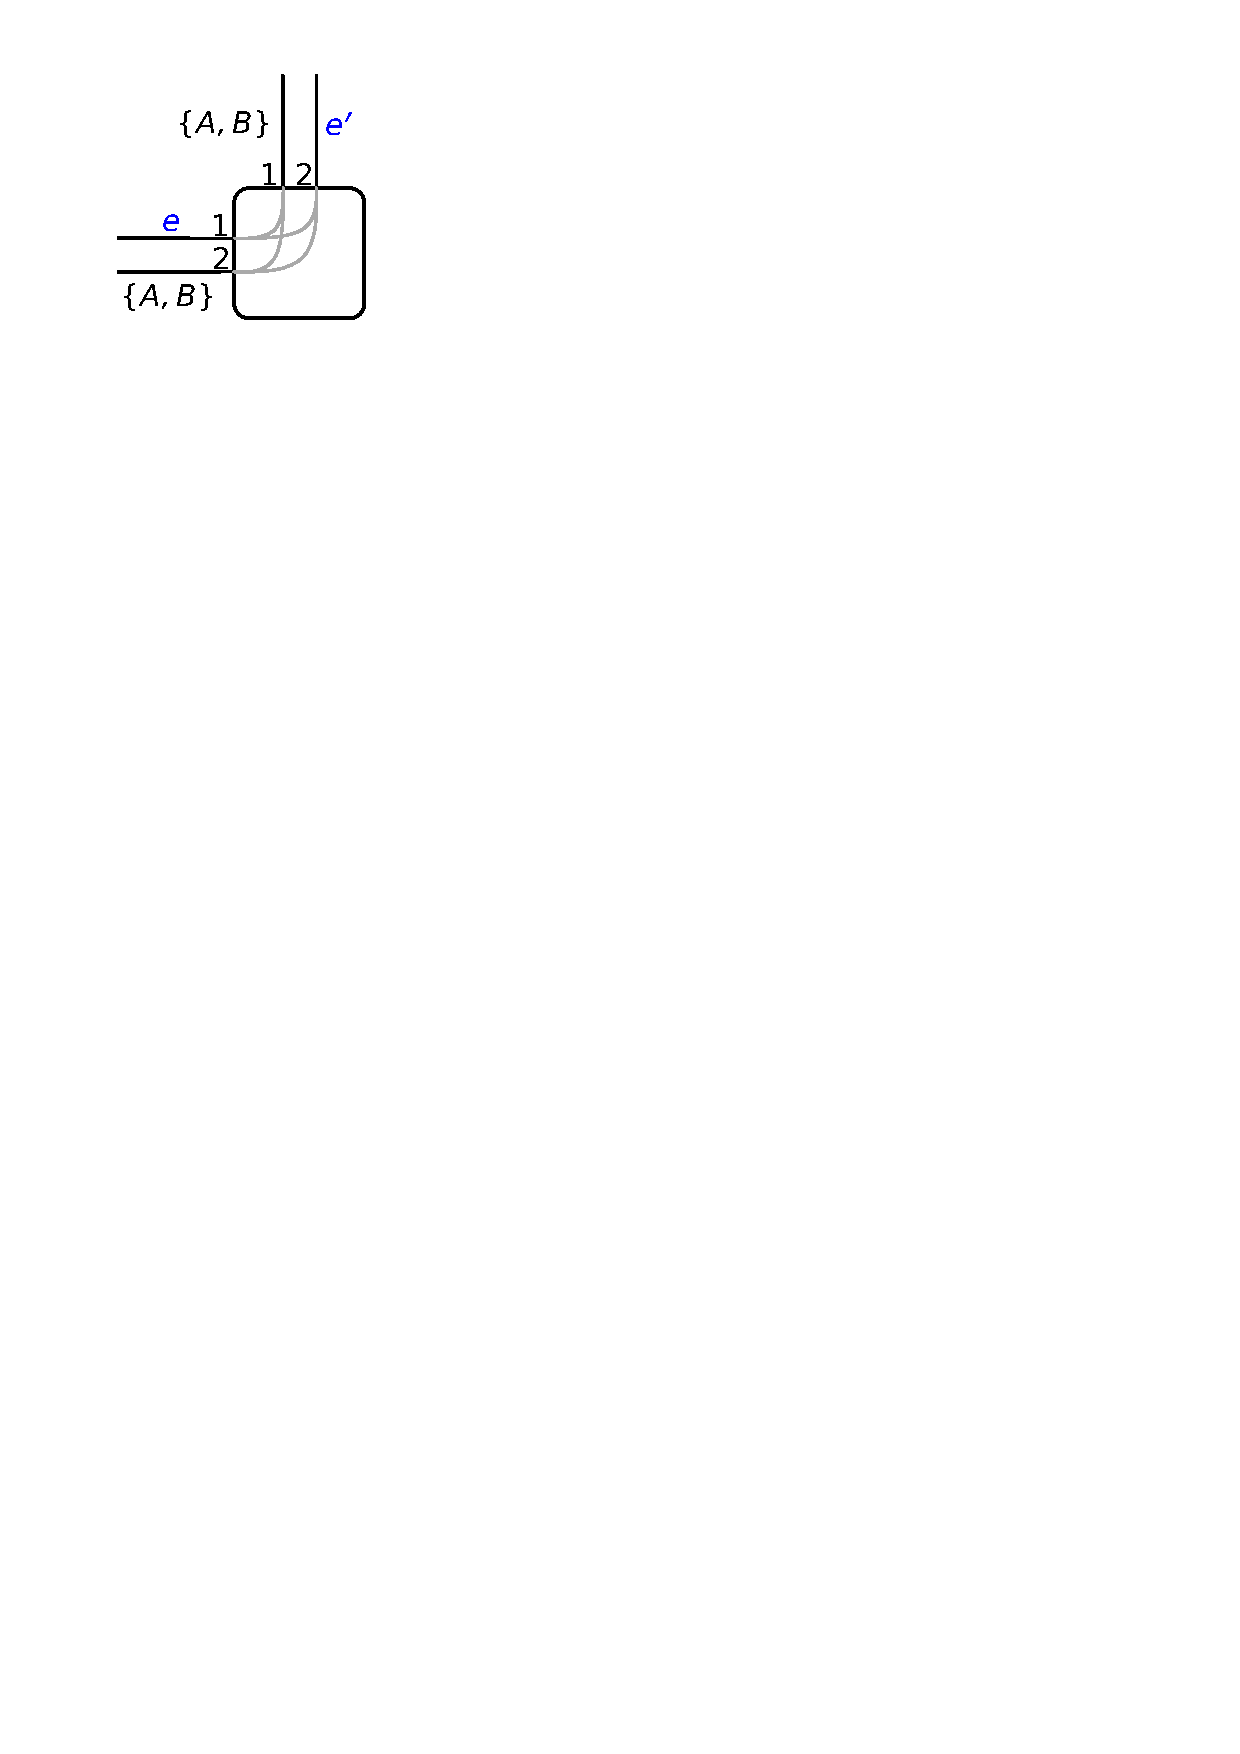
\includegraphics[width=0.9\textwidth, page=1]{figures/crossing.pdf}

			\centering\includegraphics[width=0.9\textwidth, page=2]{figures/crossing.pdf}
		\end{column}
		\begin{column}[T]{0.75\textwidth}			
			\begin{itemize}
				\item For each edge $e$, line $l$ and position $p$, introduce variable $x_{elp} \in {0, 1}$
				\item \alert{Example}: $x_{eA1}$ and $x_{eA2}$ for line $A$
				\item Constraint: all $x_{elp}$ have to sum up to 1 for a single line $l$ on a single edge $e$
				\item \alert{Standard crossing:} Objective variable $x_{ee'AB}$ which is 1 if $p_e(A) < p_{e}(B)$ and $p_{e'}(A) > p_{e'}(B)$, or else 0
				\item \alert{Split crossing:} Objective variable $x_{ee'e''AB}$ which is 1 if $p_e(A) < p_{e}(B)$, or else 0
			\end{itemize}
			\vspace{0.5cm}
			$\Rightarrow \mathcal{O}(|E|M^2)$ variables, \textcolor{red}{$\mathcal{O}(|E|M^6)$} constraints
		\end{column}
	\end{columns}
\end{frame}

% --------------------------------------------------------------------------------
\begin{frame}{Line-ordering optimization - Improved ILP}	
	\begin{itemize}
		\item \textbf{Observation:} we only need to check if $p_e(A) < p_e(B)$ (or vice versa) for both types of crossings
		\item But we explicitly enumerate all possible line positions of $A$ and $B$ on $e$
		\item \alert{Basic idea:} introduce binary variables $x_{eA<B}$ and $x_{eB<A}$ which can be efficiently checked
	\end{itemize}
	\vspace{0.5cm}
	$\Rightarrow \mathcal{O}(|E|M^2)$ variables, \textcolor{black!40!green}{$\mathcal{O}(|E|M^2)$} constraints
\end{frame}

% --------------------------------------------------------------------------------
\begin{frame}{Results so far (2)}
	\only<1>{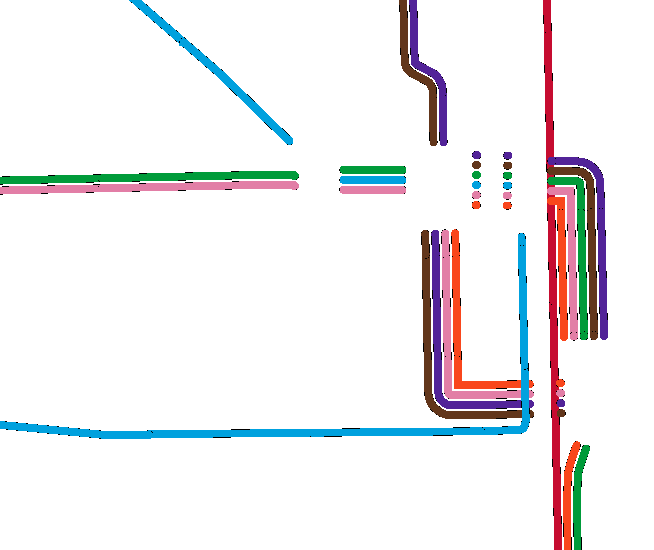
\includegraphics[width=0.8\textwidth]{figures/interim3.pdf}}
	\pause
	\only<2>{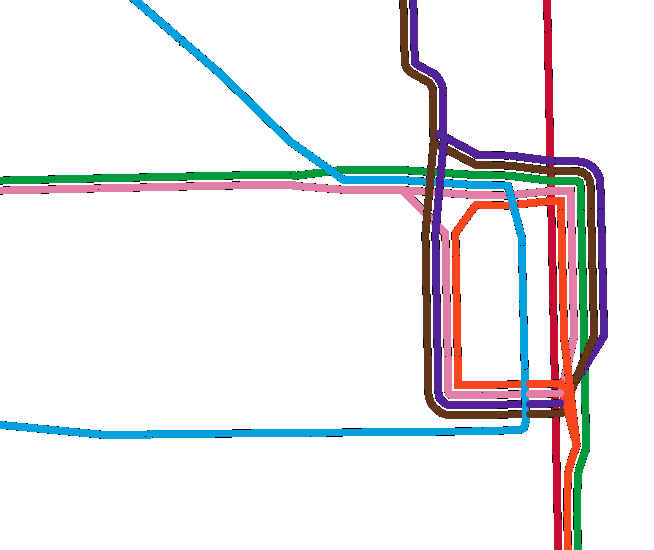
\includegraphics[width=0.8\textwidth]{figures/interim4.pdf}}
	\pause
	\only<3>{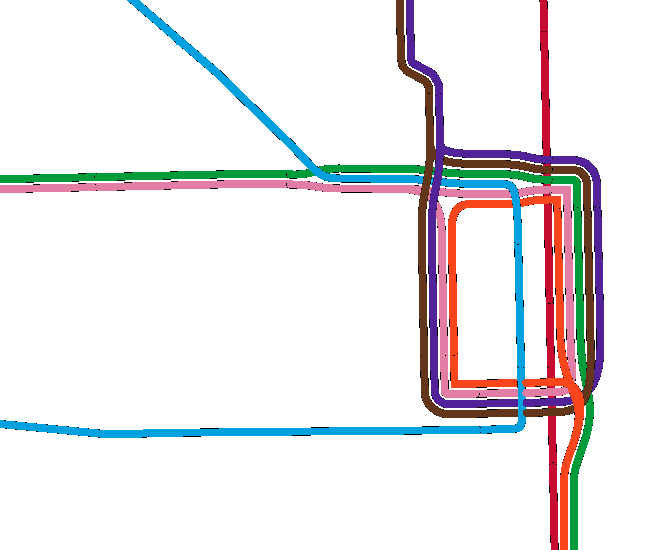
\includegraphics[width=0.804\textwidth]{figures/interim5.pdf}}
\end{frame}

% --------------------------------------------------------------------------------
\begin{frame}{Line-ordering optimization - Line separations}	
	\begin{columns}[T]
		\begin{column}[T]{0.45\textwidth}
			\centering 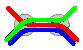
\includegraphics[width=0.7\textwidth]{figures/splitting_example_nonopt.pdf}

			1 crossing, \textcolor{red}{1 separation}

			\vspace{1.5cm}

			\centering 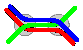
\includegraphics[width=0.7\textwidth]{figures/splitting_example2_nonopt.pdf}

			2 crossings, \textcolor{red}{1 separation}
		\end{column}
		\begin{column}[T]{0.1\textwidth}
			\centering vs

			\centering vs
		\end{column}
		\begin{column}[T]{0.45\textwidth}			
			\centering 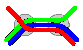
\includegraphics[width=0.7\textwidth]{figures/splitting_example.pdf}

			2 crossings, \textcolor{black!40!green}{0 separations}

			\vspace{1.5cm}

			\centering 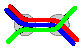
\includegraphics[width=0.7\textwidth]{figures/splitting_example2.pdf}

			2 crossings, \textcolor{black!40!green}{0 separations}
		\end{column}
	\end{columns}
\end{frame}

% --------------------------------------------------------------------------------
\begin{frame}{Line-ordering optimization - Line separations (ctd.)}	
	\begin{columns}[T]
		\begin{column}{0.25\textwidth}
			\centering\includegraphics[width=0.9\textwidth, page=3]{figures/crossing.pdf}
		\end{column}
		\begin{column}[T]{0.75\textwidth}			
			\begin{itemize}
				\item \alert{\textbf{Idea:}} If two lines $A, B$ continue from $e$ to $e'$, set a binary splitting variable $x_{ee'A\|B} = 1$ if they are next to each other in $e$, but no in $e'$
				\item Add $x_{ee'A\|B}$ to the objective function
			\end{itemize}
		\end{column}
	\end{columns}

	\vspace{1cm}
	$\Rightarrow$ Still $\mathcal{O}(|E|M^2)$ variables, $\mathcal{O}(|E|M^2)$ constraints
\end{frame}

% --------------------------------------------------------------------------------
\begin{frame}{Results so far (3)}
	\only<1>{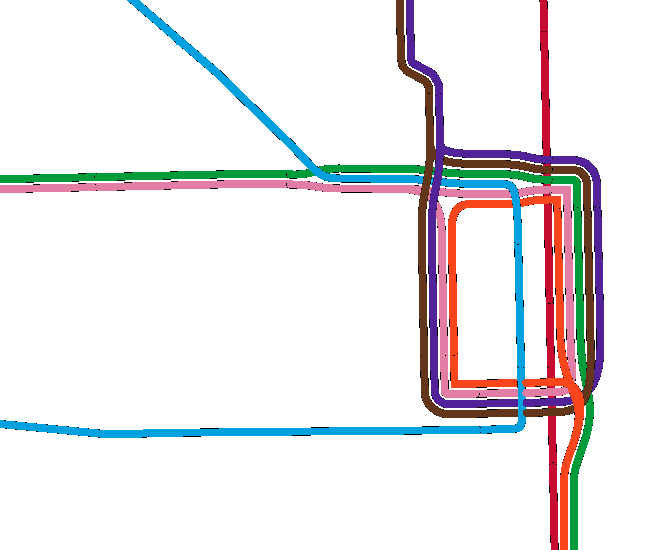
\includegraphics[width=0.804\textwidth]{figures/interim5.pdf}}
	\pause
	\only<2>{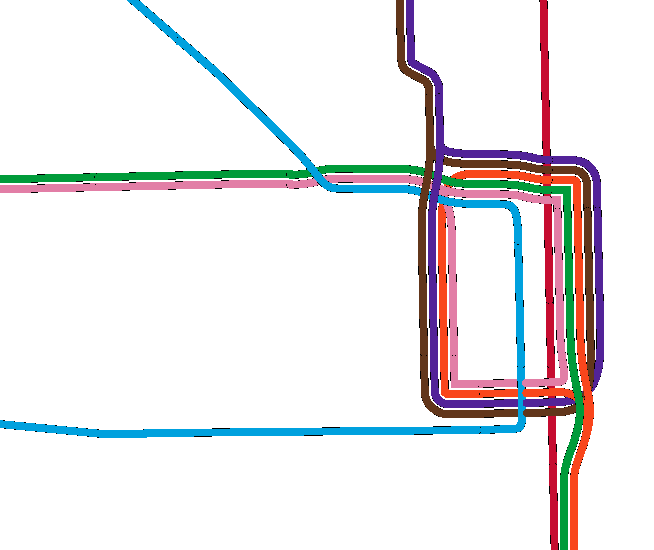
\includegraphics[width=0.804\textwidth]{figures/interim6.pdf}}
\end{frame}

% --------------------------------------------------------------------------------
\begin{frame}{Line-ordering optimization - Core optim graph}
	\centering
	\tikzstyle{graphnode}=[minimum size=14pt, inner sep=0, circle, draw=black, solid, fill=white]

	\only<1> {
		\begin{tikzpicture}[font=\small]
			\foreach \place/\x in {{(9.5, 3.8)/1}, {(11.3,3)/2},{(10.4,1.5)/3},{(9,2.3)/4}, {(8, 3.8)/5}, {(6.3, 3.3)/6}, {(8.3, 1)/7}, {(7.3, 2.5)/8}, {(6.5, 1)/9}}
			\node[graphnode] (\x) at \place {$\x$};

			\draw (1) .. controls (10.5,4) and (11, 3.7) .. (2) node [xshift=2,yshift=10, midway, below right] {$\{A,B,C\}$};
			\draw (2) .. controls (11.5,2) and (11.5, 2).. (3) node [midway, below right, xshift=-13, yshift=-5] {$\{A,B,C\}$};
			\draw (3) .. controls (9.9, 2) .. (4) node [midway, above right, yshift=-1, xshift=-4] {$\{A, B\}$};
			\draw (1) .. controls (10.3, 3) and (10.4, 2.7) .. (4) node [midway, right] {$\{C\}$};
			\draw (5) .. controls (9, 3.8) .. (1) node [xshift=-3.5, yshift=-5, midway, below] {$\{D, E, F\}$};
			\draw (4) .. controls (8, 2.3) .. (8) node [midway, below] {$\{A, B\}$};
			\draw (4) .. controls (8.6, 1.8) .. (7) node [yshift=-1, xshift=1,midway, right] {$\{E\}$};
			\draw (7) .. controls (7.35, .8) .. (9) node [midway, above] {$\{E\}$};
			\draw (9) .. controls (6.7, 2.1) .. (8) node [yshift=-3, xshift=-3, midway, below right] {$\{F\}$};
			\draw (6) .. controls (5.7, 2.3) .. (9) node [yshift=7, xshift=-1, midway, right] {$\{E,F\}$};
			\draw (6) .. controls (7.3, 3.5) .. (5) node [yshift=1, xshift=-10, midway, above] {$\{E,F\}$};
			\draw (8) .. controls (7.6, 3.3) .. (5) node [yshift=-2, xshift=-4, midway, below right] {$\{D\}$};
			\draw (7) .. controls (9.35, .8) .. (3) node [xshift=-5.5, yshift=-1, midway, above] {$\{G\}$};
		\end{tikzpicture}
	}

	\only<2> {
		\begin{tikzpicture}[font=\small]
			\foreach \place/\x in {{(9.5, 3.8)/1}, {(11.3,3)/2},{(10.4,1.5)/3},{(9,2.3)/4}, {(8, 3.8)/5}, {(6.3, 3.3)/6}, {(8.3, 1)/7}, {(7.3, 2.5)/8}, {(6.5, 1)/9}}
			\node[graphnode] (\x) at \place {$\x$};

			\draw (1) .. controls (10.5,4) and (11, 3.7) .. (2) node [xshift=2,yshift=10, midway, below right] {$\{$\textcolor{red}{$A,B$}$,C\}$};
			\draw (2) .. controls (11.5,2) and (11.5, 2).. (3) node [midway, below right, xshift=-13, yshift=-5] {$\{$\textcolor{red}{$A,B$}$,C\}$};
			\draw (3) .. controls (9.9, 2) .. (4) node [midway, above right, yshift=-1, xshift=-4] {$\{$\textcolor{red}{$A,B$}$\}$};
			\draw (1) .. controls (10.3, 3) and (10.4, 2.7) .. (4) node [midway, right] {$\{C\}$};
			\draw (5) .. controls (9, 3.8) .. (1) node [xshift=-3.5, yshift=-5, midway, below] {$\{D, E, F\}$};
			\draw (4) .. controls (8, 2.3) .. (8) node [midway, below] {$\{$\textcolor{red}{$A,B$}$\}$};
			\draw (4) .. controls (8.6, 1.8) .. (7) node [yshift=-1, xshift=1,midway, right] {$\{E\}$};
			\draw (7) .. controls (7.35, .8) .. (9) node [midway, above] {$\{E\}$};
			\draw (9) .. controls (6.7, 2.1) .. (8) node [yshift=-3, xshift=-3, midway, below right] {$\{F\}$};
			\draw (6) .. controls (5.7, 2.3) .. (9) node [yshift=7, xshift=-1, midway, right] {$\{E,F\}$};
			\draw (6) .. controls (7.3, 3.5) .. (5) node [yshift=1, xshift=-10, midway, above] {$\{E,F\}$};
			\draw (8) .. controls (7.6, 3.3) .. (5) node [yshift=-2, xshift=-4, midway, below right] {$\{D\}$};
			\draw (7) .. controls (9.35, .8) .. (3) node [xshift=-5.5, yshift=-1, midway, above] {$\{G\}$};
		\end{tikzpicture}
	}

	\only<3> {
		\begin{tikzpicture}[font=\small]			
			\node[fill=blue, circle, minimum size=18pt] at (6.3, 3.3) {};
			\node[fill=blue, circle, minimum size=18pt] at (11.3,3) {};

			\foreach \place/\x in {{(9.5, 3.8)/1}, {(11.3,3)/2},{(10.4,1.5)/3},{(9,2.3)/4}, {(8, 3.8)/5}, {(6.3, 3.3)/6}, {(8.3, 1)/7}, {(7.3, 2.5)/8}, {(6.5, 1)/9}}
			\node[graphnode] (\x) at \place {$\x$};

			\draw (1) .. controls (10.5,4) and (11, 3.7) .. (2) node [xshift=2,yshift=10, midway, below right] {$\{$\textcolor{red}{$A,B$}$,C\}$};
			\draw (2) .. controls (11.5,2) and (11.5, 2).. (3) node [midway, below right, xshift=-13, yshift=-5] {$\{$\textcolor{red}{$A,B$}$,C\}$};
			\draw (3) .. controls (9.9, 2) .. (4) node [midway, above right, yshift=-1, xshift=-4] {$\{$\textcolor{red}{$A,B$}$\}$};
			\draw (1) .. controls (10.3, 3) and (10.4, 2.7) .. (4) node [midway, right] {$\{C\}$};
			\draw (5) .. controls (9, 3.8) .. (1) node [xshift=-3.5, yshift=-5, midway, below] {$\{D, E, F\}$};
			\draw (4) .. controls (8, 2.3) .. (8) node [midway, below] {$\{$\textcolor{red}{$A,B$}$\}$};
			\draw (4) .. controls (8.6, 1.8) .. (7) node [yshift=-1, xshift=1,midway, right] {$\{E\}$};
			\draw (7) .. controls (7.35, .8) .. (9) node [midway, above] {$\{E\}$};
			\draw (9) .. controls (6.7, 2.1) .. (8) node [yshift=-3, xshift=-3, midway, below right] {$\{F\}$};
			\draw (6) .. controls (5.7, 2.3) .. (9) node [yshift=7, xshift=-1, midway, right] {$\{E,F\}$};
			\draw (6) .. controls (7.3, 3.5) .. (5) node [yshift=1, xshift=-10, midway, above] {$\{E,F\}$};
			\draw (8) .. controls (7.6, 3.3) .. (5) node [yshift=-2, xshift=-4, midway, below right] {$\{D\}$};
			\draw (7) .. controls (9.35, .8) .. (3) node [xshift=-5.5, yshift=-1, midway, above] {$\{G\}$};
		\end{tikzpicture}
	}

	\only<4> {
		\begin{tikzpicture}[font=\small]			
			\node[fill=blue, circle, minimum size=18pt] at (6.3, 3.3) {};
			\node[fill=blue, circle, minimum size=18pt] at (11.3,3) {};
			\node[fill=blue!50, circle, minimum size=18pt] at (8.3, 1) {};

			\foreach \place/\x in {{(9.5, 3.8)/1}, {(11.3,3)/2},{(10.4,1.5)/3},{(9,2.3)/4}, {(8, 3.8)/5}, {(6.3, 3.3)/6}, {(8.3, 1)/7}, {(7.3, 2.5)/8}, {(6.5, 1)/9}}
			\node[graphnode] (\x) at \place {$\x$};

			\draw (1) .. controls (10.5,4) and (11, 3.7) .. (2) node [xshift=2,yshift=10, midway, below right] {$\{$\textcolor{red}{$A,B$}$,C\}$};
			\draw (2) .. controls (11.5,2) and (11.5, 2).. (3) node [midway, below right, xshift=-13, yshift=-5] {$\{$\textcolor{red}{$A,B$}$,C\}$};
			\draw (3) .. controls (9.9, 2) .. (4) node [midway, above right, yshift=-1, xshift=-4] {$\{$\textcolor{red}{$A,B$}$\}$};
			\draw (1) .. controls (10.3, 3) and (10.4, 2.7) .. (4) node [midway, right] {$\{C\}$};
			\draw (5) .. controls (9, 3.8) .. (1) node [xshift=-3.5, yshift=-5, midway, below] {$\{D, E, F\}$};
			\draw (4) .. controls (8, 2.3) .. (8) node [midway, below] {$\{$\textcolor{red}{$A,B$}$\}$};
			\draw (4) .. controls (8.6, 1.8) .. (7) node [yshift=-1, xshift=1,midway, right] {$\{E\}$};
			\draw (7) .. controls (7.35, .8) .. (9) node [midway, above] {$\{E\}$};
			\draw (9) .. controls (6.7, 2.1) .. (8) node [yshift=-3, xshift=-3, midway, below right] {$\{F\}$};
			\draw (6) .. controls (5.7, 2.3) .. (9) node [yshift=7, xshift=-1, midway, right] {$\{E,F\}$};
			\draw (6) .. controls (7.3, 3.5) .. (5) node [yshift=1, xshift=-10, midway, above] {$\{E,F\}$};
			\draw (8) .. controls (7.6, 3.3) .. (5) node [yshift=-2, xshift=-4, midway, below right] {$\{D\}$};
			\draw (7) .. controls (9.35, .8) .. (3) [draw=black!30!green, line width=2pt] node [xshift=-5.5, yshift=-1, midway, above] {$\{G\}$};
		\end{tikzpicture}
	}

	\only<5> {
		\begin{tikzpicture}[font=\small]
			\foreach \place/\x in {{(9.5,4)/1}, {(10.3,2.3)/3},{(9,2.3)/4}, {(7, 4)/5}, {(8.1, 3.1)/8}, {(6.5, 2)/9}}
			\node[graphnode] (\x) at \place {$\x$};

			\draw (1) -- (3) node [midway, above right] {$\{X,C\}$};
			\draw (3) -- (4) node [midway, below] {$\{X\}$};
			\draw (1) -- (4) node [midway, below right, xshift=-2pt, yshift=4pt] {$\{C\}$};
			\draw (5) -- (1) node [midway, above] {$\{D,E,F\}$};
			\draw (4) -- (8) node [midway, below left, yshift=3pt, xshift=2pt] {$\{X\}$};
			\draw (4) -- (9) node [midway, below right] {$\{E\}$};
			\draw (9) -- (8) node [midway, above, yshift=3pt] {$\{F\}$};
			\draw (5) -- (9) node [midway, above left] {$\{E,F\}$};
			\draw (8) -- (5) node [midway, right, xshift=1pt, yshift=2pt] {$\{D\}$};
		\end{tikzpicture}
	}

	\only<6> {
		\begin{tikzpicture}[font=\small]
			\foreach \place/\x in {{(9.5,4)/1}, {(10.3,2.3)/3},{(9,2.3)/4}, {(7, 4)/5}, {(8.1, 3.1)/8}, {(6.5, 2)/9}}
			\node[graphnode] (\x) at \place {$\x$};

			\draw (1) -- (3) node [midway, above right] {$\{X,C\}$};
			\draw (3) -- (4) [draw=blue!40!red, line width=2pt] node [midway, below] {$\{X\}$};
			\draw (1) -- (4) [draw=blue!40!red, line width=2pt] node [midway, below right, xshift=-2pt, yshift=4pt] {$\{C\}$};
			\draw (5) -- (1) node [midway, above] {$\{D,E,F\}$};
			\draw (4) -- (8) node [midway, below left, yshift=3pt, xshift=2pt] {$\{X\}$};
			\draw (4) -- (9) [draw=blue!40!red, line width=2pt]  node [midway, below right] {$\{E\}$};
			\draw (9) -- (8) [draw=blue!40!red, line width=2pt] node [midway, above, yshift=3pt] {$\{F\}$};
			\draw (5) -- (9) node [midway, above left] {$\{E,F\}$};
			\draw (8) -- (5) [draw=blue!40!red, line width=2pt] node [midway, right, xshift=1pt, yshift=2pt] {$\{D\}$};
		\end{tikzpicture}
	}

	\only<7> {
		\tikzstyle{graphnode}=[minimum size=14pt, inner sep=0, circle, draw=black, solid, fill=white]
		\tikzstyle{connnode}=[minimum size=6pt, inner sep=0, circle, draw=black, solid, fill=white]
		\begin{tikzpicture}[font=\small]
			\foreach \place/\x in {{(10.1,3.7)/1}, {(10.9,2)/3}, {(7, 3.7)/5}, {(6.5, 2)/9}}
			\node[graphnode] (\x) at \place {$\x$};

			\foreach \place/\x in {{(8, 3.7)/11}, {(9.6,2)/4}, {(9.9,2.7)/41}, {(7.8, 2.9)/13}, {(7.8, 2.5)/14}, {(8,2.1)/15}}
			\node[connnode] (\x) at \place {};

			\draw (1) -- (3) node [midway, above right] {$\{X,C\}$};
			\draw (3) -- (4) node [midway, below] {$\{X\}$};
			\draw (1) -- (41) node [midway, left, xshift=0pt, yshift=1pt] {$\{C\}$};

			\draw (5) -- (9) node [midway, above left] {$\{E,F\}$};

			\draw (13) -- (5) node [midway, right, xshift=1pt, yshift=0pt] {$\{D\}$};
			\draw (9) -- (14) node [midway, above, yshift=3pt] {$\{F\}$};

			\draw (15) -- (9) node [midway, below right] {$\{E\}$};

			\draw (5) -- (11) node [midway, above, yshift=4pt] {$\{D,E,F\}$};
		\end{tikzpicture}
	}

	\pause

	\begin{itemize}[<+->]
		\item Combine lines \textcolor{red}{$A,B$} that \alert{always occur together} into a single new line ($A,B \rightarrow X$)
		\item Delete \textcolor{blue}{nodes with degree 2} and merge their adjacent edges
		\item Remove edges \textcolor{black!30!green}{$(u, v)$} where $u$ and $v$ are \alert{termini} for all $L((u, v))$\pause
		\item Cut \textcolor{blue!40!red}{edges} with $|L(e)| = 1$
	\end{itemize}
\end{frame}

% --------------------------------------------------------------------------------
\begin{frame}{Rendering}
	% TODO: maybe numbering? or arrows?
	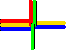
\includegraphics[width=0.35\textwidth]{figures/render_example1.pdf}\hfill
	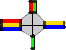
\includegraphics[width=0.35\textwidth]{figures/render_example2.pdf}

	\vspace{1cm}

	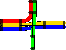
\includegraphics[width=0.35\textwidth]{figures/render_example3.pdf}\hfill
	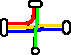
\includegraphics[width=0.35\textwidth]{figures/render_example4.pdf}
\end{frame}

% --------------------------------------------------------------------------------
\begin{frame}{Results so far (4)}	
	\only<1>{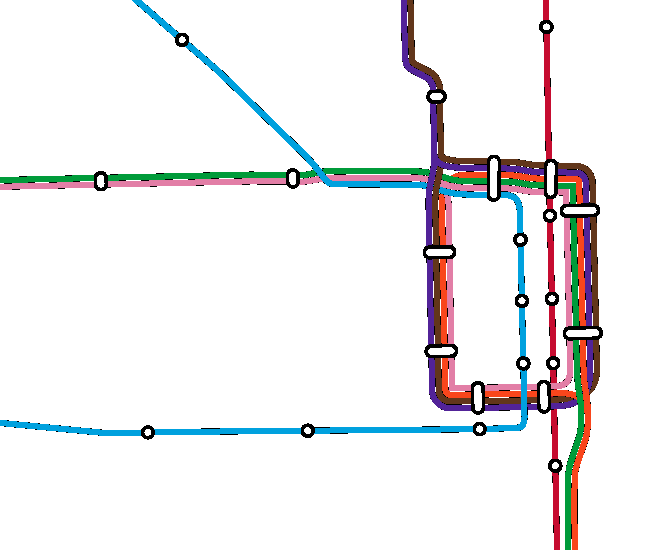
\includegraphics[width=0.9\textwidth]{figures/final.pdf}}
\end{frame}

% --------------------------------------------------------------------------------
\begin{frame}{Evaluation}	
	% TODO
\end{frame}

% --------------------------------------------------------------------------------
\begin{frame}{Future work}	
	\begin{itemize}
		\item Additional rules for core graph reduction \alert{(work in progress)}
		\item Faster construction times of line graph
		\item TODO
	\end{itemize}
\end{frame}

% --------------------------------------------------------------------------------
\begin{frame}{}	
	\centering \huge Thank you!
\end{frame}

\end{document}
